% command to make sure colorboxes don't create whitespace between code lines
\fboxsep=.6pt

% default settings for listings
\lstset{style=python}

\title[Programmieren]{Programmieren: Bubble Sort (Datenstrukturen)}

\subtitle{Listen}

\author[Wendl, Cyril] % (optional)
{Cyril Wendl}

\institute[KLW] % (optional)
{
	Fachschaft Informatik\\
	Kantonsschule im Lee
}

\date[\today] % (optional)

\logo{
\includegraphics[width=2cm]{Logos/LeeLogo}}

\titlegraphic{\vspace{-.7cm}\includegraphics[width=\textwidth]{"Grundlagen_Info/06_Datenbanken/Figures/title-emojis"}}

\frame{\titlepage}

\newcommand{\includesteps}[1]{%
	\foreach \step in {1,...,#1}{%
			\only<\step>{%
				\begin{figure}[H]
					\input{Grundlagen_Info/00_Programmieren/Skript/Code/K06_Datenstrukturen/tikz/bubble_sort_steps/step_\step.tex}
				\end{figure}
			}%
		}
}

\begin{frame}[fragile]{Sortier-Algorithmen}
	Wie kommen wir von \lstinline|x = [5, 3, 8, 20, 2, 10]|	zu \lstinline|x = [2, 3, 5, 8, 10, 20]|?
	\begin{itemize}[<+->]
		\item \textbf{Algorithmus} = \textit{eindeutige} und \textit{endliche} Abfolge von Anweisungen oder Schritten zur Lösung eines Problems
		\item \textbf{Sortieren}: Wichtig, um Daten zu organisieren, Zugriff und die Suche nach Elementen effizienter zu machen und bildet die Grundlage für viele weitere Anwendungen und Algorithmen (z.B. \textit{Suche}).
		      \begin{figure}[H]
			      \centering
			      \raisebox{-0.5\height}{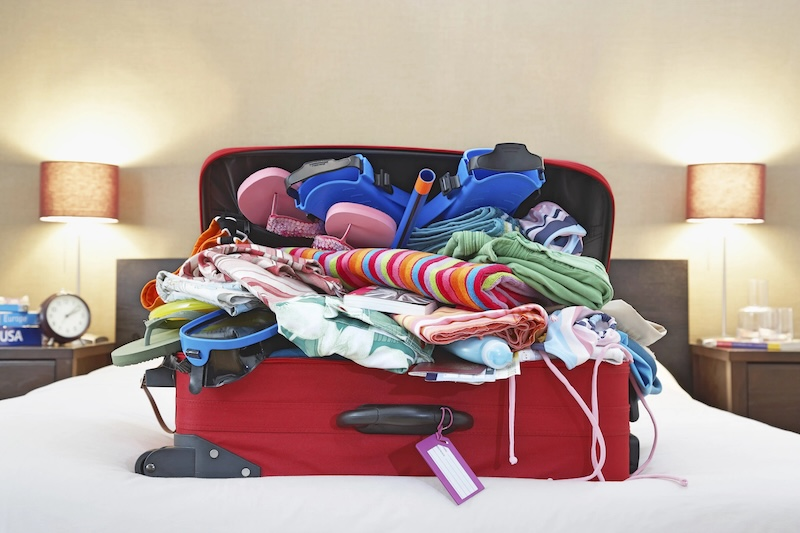
\includegraphics[width=.3\textwidth]{Grundlagen_Info/04_Kompression/Figures/messy_suitcase.jpg}}
			      \raisebox{-0.5\height}{$\rightarrow$}
			      \raisebox{-0.5\height}{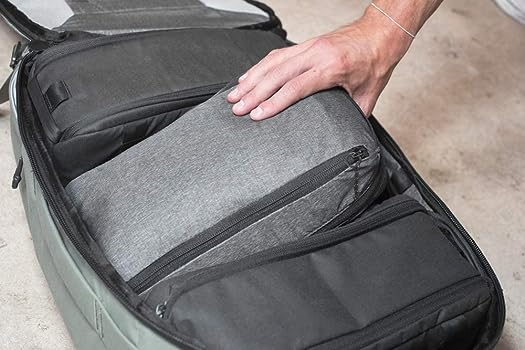
\includegraphics[width=.3\textwidth]{Grundlagen_Info/00_Programmieren/Figures/prog-packing-cubes}}
		      \end{figure}
	\end{itemize}

	\only<3->{Heute: \textbf{Bubble-Sort-Algorithmus}}
\end{frame}

% Replace <number_of_steps>tete with the actual number of steps generated
\begin{frame}[fragile]{Bubble-Sort-Algorithmus}{Visualisierung}
	\includesteps{36}
\end{frame}

\begin{frame}[fragile]{Bubble-Sort-Algorithmus}{Python-Code}
	Bevor wir uns den Algorithmus anschauen... Kann man Listen-Elemente so vertauschen?
	\begin{lstlisting}
# x ist die Liste, die sortiert werden soll
x = [5, 3, 8, 20, 2, 10]

x[0] = x[1]
print(x) # wie sieht die Liste jetzt aus?

x[1] = x[0]
print(x) # wie sieht die Liste jetzt aus?
	\end{lstlisting}
\end{frame}

\begin{frame}[fragile]{Bubble-Sort-Algorithmus}{Python-Code}
	Wir brauchen einen Zwischenspeicher!
	\begin{lstlisting}[basicstyle=\footnotesize\ttfamily]
# x ist die Liste, die sortiert werden soll
x = [5, 3, 8, 20, 2, 10]

# Zwischenspeicher-Variable a erstellen *bevor* wir x[0] überschreiben
a = x[0] 

# Das erste Element von x wird überschrieben durch den zweiten Wert von x (wir verlieren also den ersten Wert, haben ihn aber noch in a als "Backup" in a gespeichert)
x[0] = x[1]
print(x)

# Jetzt können wir das "Backup" in das zweite Element  von x einfügen
x[1] = a
print(x)
	\end{lstlisting}
\end{frame}

\begin{frame}[fragile]{Bubble-Sort-Algorithmus: Python-Code}
	\begin{lstlisting}[basicstyle=\small\ttfamily]
# x ist die Liste, die sortiert werden soll
x = [5, 3, 8, 20, 2, 10]

for _ in range(len(x) - 1):
    i = 0
	for _ in range(len(x) - 1):
    	# falls falsche Reihenfolge, dann...
        if x[i] > x[i + 1]:
			# ...Tausch von x[i] und x[i + 1]
            z = x [i]
            x[i] = x[i + 1]
            x[i + 1] = z

        i += 1
    print(x)
	\end{lstlisting}
\end{frame}

\begin{frame}[fragile]{Bubble-Sort-Algorithmus: Python-Code (\textbf{optimiert})}
	\begin{lstlisting}[basicstyle=\small\ttfamily]
# x ist die Liste, die sortiert werden soll
x = [5, 3, 8, 20, 2, 10]

i = 0
for _ in range(len(x) - 1):
    j = 0
	for _ in range(len(x) - 1 -i):
    	# falls falsche Reihenfolge, dann...
        if x[j] > x[j + 1]:
			# ...Tausch von x[j] und x[j + 1]
            z = x [j]
            x[j] = x[j + 1]
            x[j + 1] = z

        j += 1
    print(x)
	i += 1
	\end{lstlisting}
\end{frame}

\begin{frame}[fragile]{Laufzeit des Algorithmus}
	Anzahl Vergleiche, falls die Liste $n$ lang ist
	\begin{itemize}[<+->]
		\item Allgemein
		      \begin{itemize}
			      \item Nicht optimierte Version:
			            \[(n-1)^2\]
			      \item Optimierte Version:
			            \[\sum_{m=1}^{n-1}m \]
		      \end{itemize}
		\item Also z.B., falls Liste 6 Elemente enthält
		      \begin{itemize}
			      \item Nicht optimierte Version: $5^2 = 25$ Vergleiche
			      \item Optimierte Version: $\displaystyle\sum_{m=1}^{5}m = 1 + 2 + 3 + 4 + 5 = 15$ Vergleiche
		      \end{itemize}
	\end{itemize}
\end{frame}


\begin{frame}[fragile]{Auftrag}
	\begin{itemize}
		\item Moodle-Aufgaben ``Bubble Sort''
		\item \aufgabebox{Aufgabe 6.12}
	\end{itemize}
\end{frame}

